% !TEX program = xelatex
%% =====================================================================
%%  VZOR maturitní práce – Gymnázium Jírovcova 8, České Budějovice
%%  Autoři šablony: Jonáš Havelka, Michal Kočer, Daniel Sýkora (MIT)
%% =====================================================================
%%  Tento dokument ukazuje, jak vypadá hotová práce a jak se sázejí
%%  jednotlivé prvky. Svou práci pište do souboru mprace.tex.
%%
%%  Hotové PDF: vzor.pdf. Zdroje ukázek: vzor/ukazky/*.tex
%%  (pod každou ukázkou je v PDF šedě uvedeno, ve kterém souboru je).
%%
%%  Kostra tohoto souboru odpovídá souboru mprace.tex (hlídá make check).
%%  Vzor obsahuje mnoho obrázků a diagramů – na Overleafu (zdarma) by
%%  se nemusel stihnout přeložit; překládejte ho lokálně: make vzor
%% =====================================================================
\documentclass[12pt]{report}
\usepackage{MP}								% Styl maturitní práce
\addbibresource{vzor/vzor.bib}				% Soubor se seznamem literatury

%% Balíčky, které jsou v mprace.tex volitelné (vzor je potřebuje pro ukázky)
\usepackage{tikz}\usetikzlibrary{arrows.meta,shapes.geometric,positioning} % diagramy, schémata
\usepackage[version=4]{mhchem}				% chemické vzorce \ce{...}
\usepackage{lipsum}							% výplňový text vzoru

\graphicspath{{images/}{vzor/obrazky/}}		% Obrázky vzoru jsou ve vzor/obrazky
\newcommand{\zdrojukazky}[1]{%				% Poznámka, kde je zdroj ukázky
	\par\noindent{\small\color{gray}Zdroj ukázky: \texttt{#1}}\par\medskip}

%% ---------------------------------------------------------------------
%%  ÚDAJE O PRÁCI
%% ---------------------------------------------------------------------
\author{Arnošt Thor}						% Jméno a příjmení
\title{Jak psát práci v \LaTeX{}u}			% Název práce
\date{14. února 2027}						% Datum odevzdání
\vedouci{Mgr. František Kantor, PhD.}		% Vedoucí práce i s tituly
\place{V Českých Budějovicích}
\skolnirok{2026/2027}
\logo{
\includegraphics[scale=1.25]{GJ8_logotyp}}

\begin{document}
%% ---- ÚVODNÍ STRANY (číslováno římsky, čísla stran se nezobrazují) ----
\pagenumbering{roman}
\mytitlepage

\prohlaseni{
	Prohlašuji, že jsem tuto práci vypracoval samostatně s vyznačením všech použitých pramenů.

	% Pokud jste při psaní práce využili nástroje umělé inteligence, uveďte to zde.
	% Smažte nebo upravte následující větu dle skutečnosti:
	Pro kontrolu pravopisu, úpravu formulací a generování komentářů ke zdrojovým textům
	jsem využil nástroj umělé inteligence Claude Sonnet (Anthropic).
	Veškerý obsah práce jsem vytvořil samostatně; nástroj sloužil výhradně jako pomocný prostředek.
}

\abstrakt{
	\lipsum[1]
}{
	latex, typografie, maturitní práce, šablona, XeLaTeX
}

\podekovani{
	\lipsum[2]
}

{\tableofcontents\newpage}

%% ---- VLASTNÍ PRÁCE (číslováno arabsky) ----
\pagenumbering{arabic}

% !TEX root = ../../vzor.tex
%% Úvod vzoru – vysvětluje, jak se šablonou pracovat.
\chapter*{Úvod}
\addcontentsline{toc}{chapter}{Úvod}

Tato šablona slouží k psaní maturitní práce na Gymnáziu Jírovcova 8 v Českých Budějovicích.
Dokument, který právě čtete, je \emph{vzor}: ukazuje, jak vypadá hotová práce
a jak se v \LaTeX{}u sázejí jednotlivé prvky -- citace, rovnice, obrázky, tabulky,
diagramy nebo výpisy programů.
Pod nadpisem každé ukázky je šedě uvedeno, ve kterém souboru najdete její zdrojový kód
(všechny ukázky jsou ve složce \texttt{vzor/ukazky/}).

Svou práci pište do souboru \texttt{mprace.tex} a do souborů ve složce \texttt{kapitoly/}:
\begin{itemize}
	\item \texttt{mprace.tex} -- údaje o práci, úvodní strany a pořadí kapitol,
	\item \texttt{kapitoly/uvod.tex}, \texttt{teorie.tex}, \texttt{prakticka.tex}, \texttt{zaver.tex}
	      a \texttt{prilohy.tex} -- vlastní text práce,
	\item \texttt{Bibliografie.bib} -- seznam literatury,
	\item \texttt{images/} -- obrázky.
\end{itemize}

\textbf{Než začnete psát, vyplňte v souboru \texttt{mprace.tex} údaje o práci:}
\begin{itemize}
	\item \verb|\author{Jméno Příjmení}| \quad -- vaše jméno a příjmení
	\item \verb|\title{Název práce}| \quad -- úplný název vaší maturitní práce
	\item \verb|\date{datum odevzdání}| \quad -- datum odevzdání, např.~\texttt{14.~února~2027}
	\item \verb|\vedouci{Mgr. Jméno Příjmení}| \quad -- jméno vedoucího práce s titulem
	\item \verb|\skolnirok{2026/2027}| \quad -- aktuální školní rok
\end{itemize}

Práci překládejte \textbf{XeLaTeXem} (na Overleafu: \emph{Menu $\to$ Compiler $\to$ XeLaTeX}).
Jak šablonu použít na Overleafu, v GitHub Codespaces nebo na vlastním počítači,
popisuje soubor \texttt{README.md} v~repozitáři šablony
\url{https://github.com/gymji/MaturitniPraceLaTeXvzor}.


\part{Teoretická část}						% Přejmenujte podle obsahu práce
% !TEX root = ../../vzor.tex
%% Teoretická část vzoru – jednotlivé ukázky jsou ve vzor/ukazky/.
\chapter{Název úvodní kapitoly}

% !TEX root = ../../vzor.tex
%% Ukázka: citace, české uvozovky, tabulka
%% Vkládá ji soubor vzor/kapitoly/teorie.tex; ve vzor.pdf je pod nadpisem uvedeno „Zdroj ukázky".

\section{Citace}
\zdrojukazky{vzor/ukazky/citace.tex}
	Odkaz v závorkách: \parencite[viz][str. 900]{einstein}\\
	Odkaz: \cite{knuthwebsite}\\
	A odkaz pod čarou: \footcite[viz][str. 42]{latexcompanion}\\
	Odkaz na českou knihu: \cite{mareks}\\
	České uvozovky se sází příkazem \verb|\uv{text}|, například: \uv{příliš žluťoučký kůň úpěl ďábelské ódy}.\\
	Inline matematický výraz: $a^2 + b^2 = c^2$ nebo $\sum_{i=1}^{n} i = \frac{n(n+1)}{2}$.
	
	\begin{table}[htbp]
		\centering
		\caption{Naměřené hodnoty rychlosti}
		\label{tab:mereni}
		\begin{tabular}{lcc}
			\toprule
			Měření & Čas $t$ [\si{\second}] & Rychlost $v$ [\si{\meter\per\second}] \\
			\midrule
			1 & 1{,}25 & 3{,}84 \\
			2 & 1{,}30 & 3{,}69 \\
			3 & 1{,}22 & 3{,}93 \\
			\midrule
			Průměr & 1{,}26 & 3{,}82 \\
			\bottomrule
		\end{tabular}
	\end{table}

\lipsum[2]

% !TEX root = ../../vzor.tex
%% Ukázka: číslované rovnice, align, řecká písmena, vektory
%% Vkládá ji soubor vzor/kapitoly/teorie.tex; ve vzor.pdf je pod nadpisem uvedeno „Zdroj ukázky".

\section{Matematické výrazy}
\zdrojukazky{vzor/ukazky/matematika.tex}

Číslovaná rovnice se vytvoří prostředím \texttt{equation}; odkazujeme na ni příkazem \verb|\eqref{}|.
Pythagorova věta~\eqref{eq:pythagoras}:
\begin{equation}
	a^2 + b^2 = c^2
	\label{eq:pythagoras}
\end{equation}

Víceřádkové odvození se zarovnaným rovnítkem (prostředí \texttt{align}):
\begin{align}
	E         &= mc^2 \\
	\vec{F}   &= m\vec{a} \\
	W         &= \vec{F} \cdot \vec{s}
\end{align}

Příklady zápisů v textu: řecká písmena $\alpha, \beta, \omega, \Delta, \lambda$,
integrál $\int_a^b f(x)\,dx$, parciální derivace $\frac{\partial f}{\partial x}$,
vektory $\vec{F}$, normálový vektor $\hat{n}$.

% !TEX root = ../../vzor.tex
%% Ukázka: obrázky: wrapfigure, figure, subfigure; krátký název sekce
%% Vkládá ji soubor vzor/kapitoly/teorie.tex; ve vzor.pdf je pod nadpisem uvedeno „Zdroj ukázky".

\section[Obrázky]{Obrázky (ukázka krátkého názvu sekce v obsahu)}
%%% v obsahu se zobrazí jen text v hranatých závorkách – hodí se pro dlouhé nadpisy
\zdrojukazky{vzor/ukazky/obrazky.tex}

Obrázek s obtékáním textu – balíček \texttt{wrapfig} (obrázek~\ref{fig:wrap}):
\begin{wrapfigure}{r}{0.4\linewidth}
	\centering
	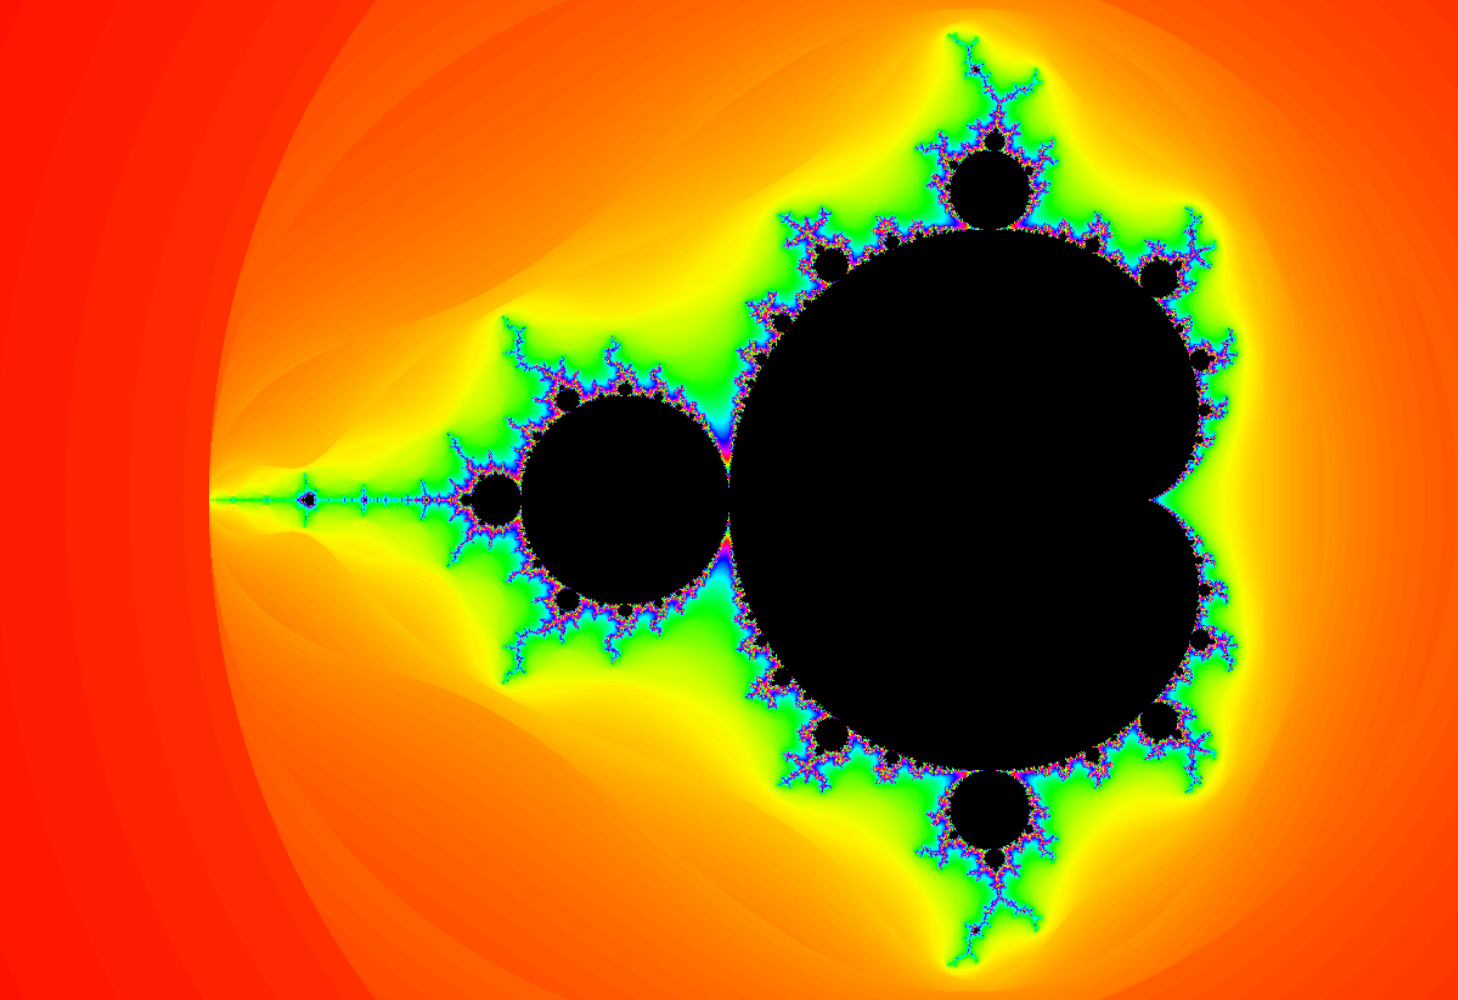
\includegraphics[width=\linewidth]{mandelbrot}
	\caption{Mandelbrotova množina}
	\label{fig:wrap}
\end{wrapfigure}
\lipsum[5]

Standardní obrázek přes celou šíři textu (obrázek~\ref{fig:test}):
\begin{figure}[htbp]
	\centering
	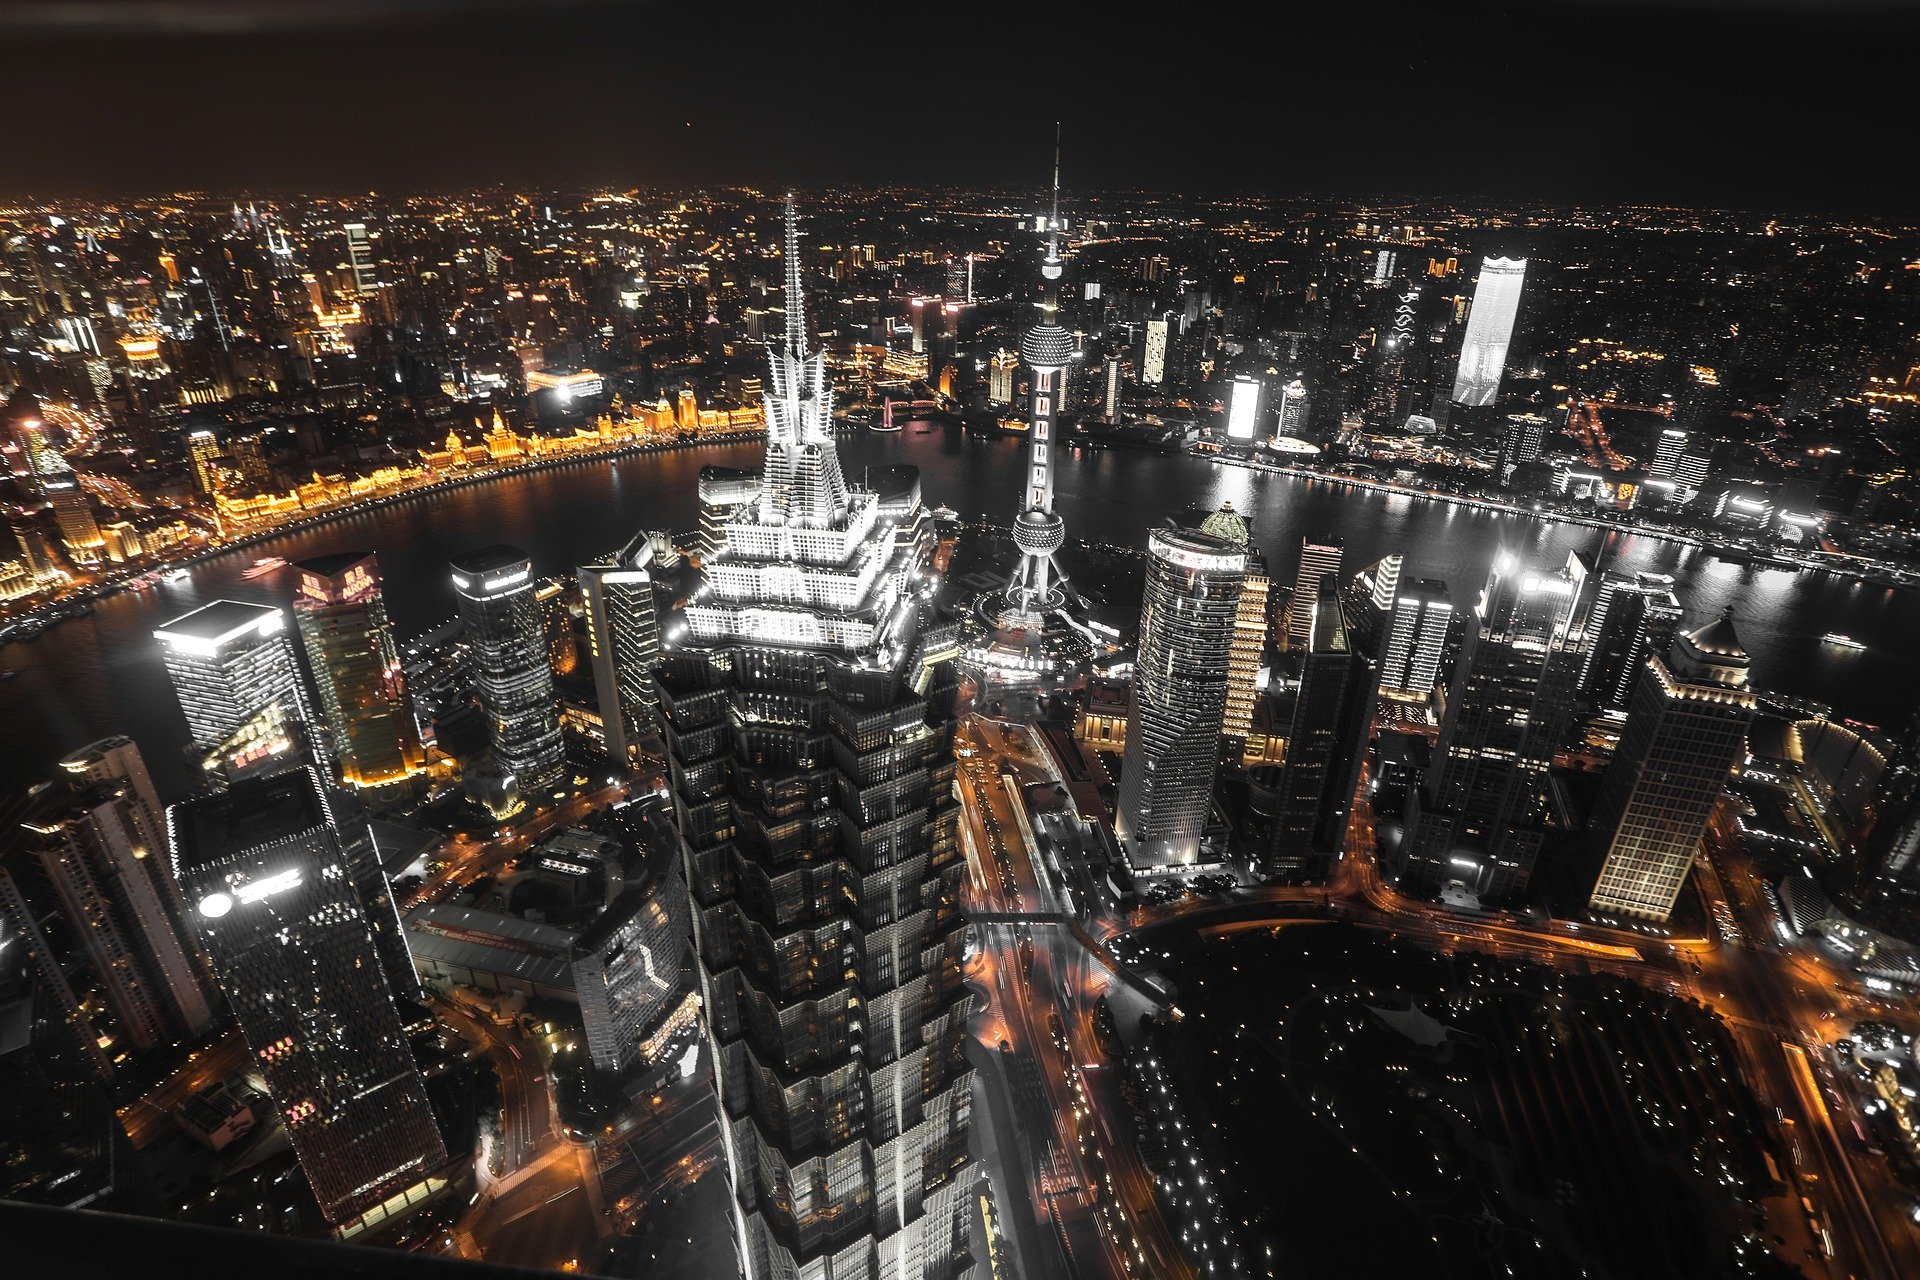
\includegraphics[width=\linewidth]{test.jpg}
	\caption{Šanghaj, zdroj: Pixabay}
	\label{fig:test}
\end{figure}

Tabulka~\ref{tab:mereni} obsahuje naměřené hodnoty.

\lipsum[3-5]

Dva obrázky vedle sebe – balíček \texttt{subcaption} (obrázky~\ref{fig:sub1} a~\ref{fig:sub2}):
\begin{figure}[htbp]
	\centering
	\begin{subfigure}{0.48\linewidth}
		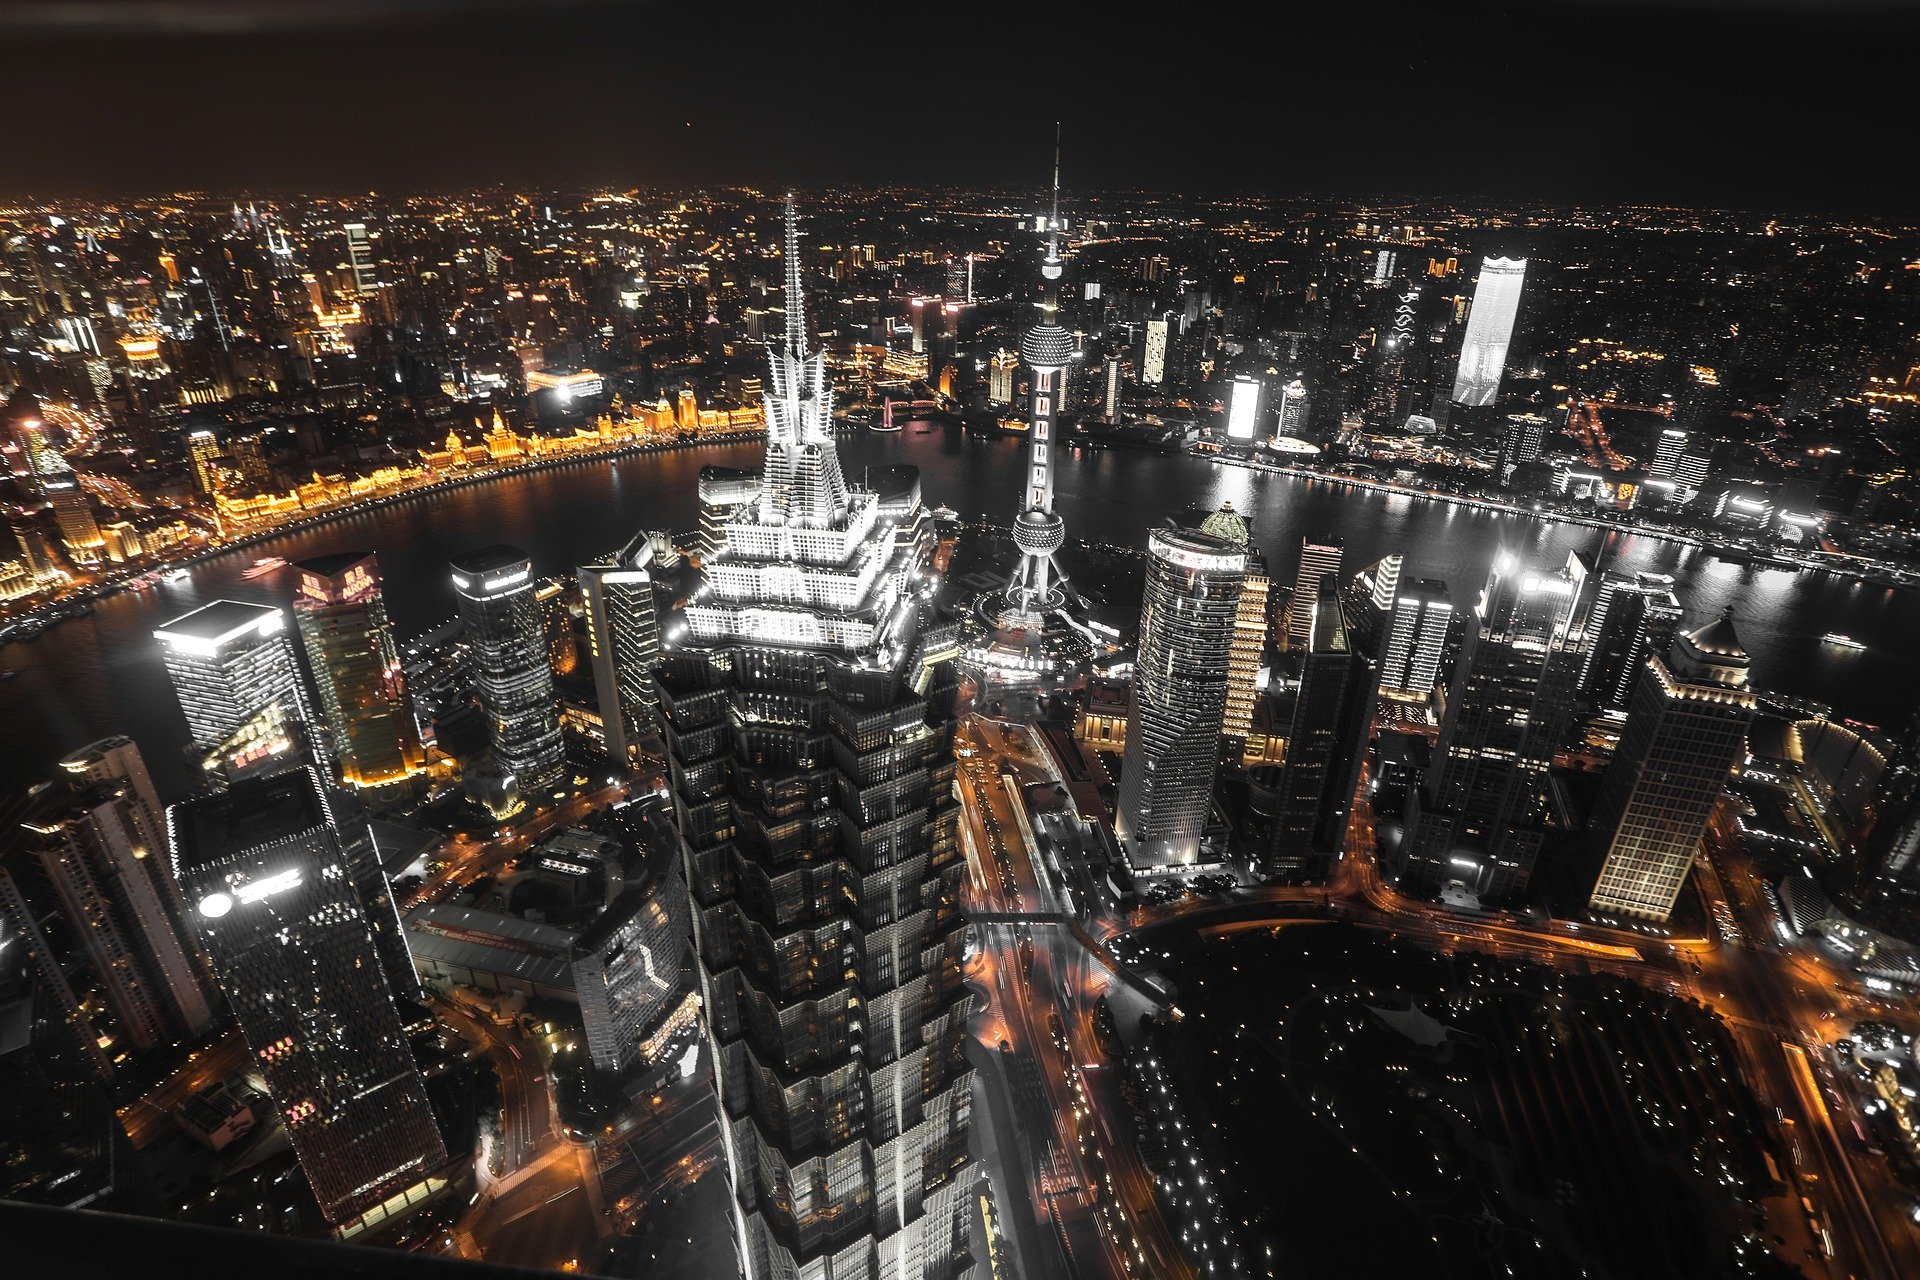
\includegraphics[width=\linewidth]{test.jpg}
		\caption{Šanghaj (Pixabay)}
		\label{fig:sub1}
	\end{subfigure}
	\hfill
	\begin{subfigure}{0.48\linewidth}
		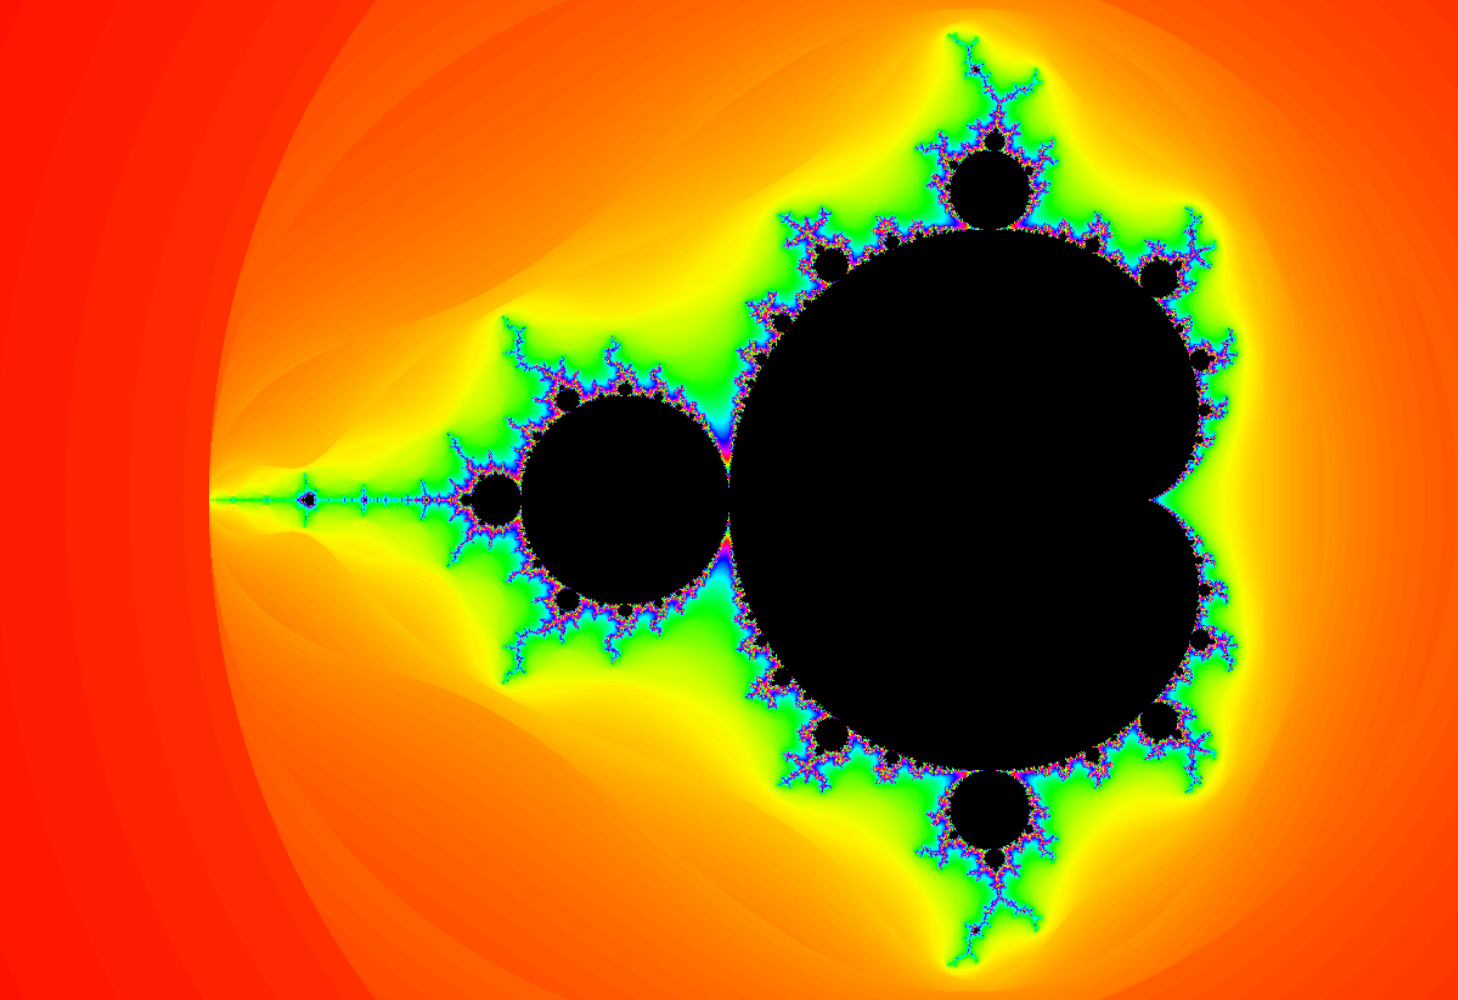
\includegraphics[width=\linewidth]{mandelbrot}
		\caption{Mandelbrotova množina}
		\label{fig:sub2}
	\end{subfigure}
	\caption{Dva obrázky vedle sebe}
	\label{fig:subfig}
\end{figure}

\lipsum[6]



\part{Praktická část}						% Přejmenujte podle obsahu práce
% !TEX root = ../../vzor.tex
%% Praktická část vzoru – jednotlivé ukázky jsou ve vzor/ukazky/.
\chapter{Název kapitoly praktické části}

% !TEX root = ../../vzor.tex
%% Ukázka: jednotky SI (siunitx)
%% Vkládá ji soubor vzor/kapitoly/prakticka.tex; ve vzor.pdf je pod nadpisem uvedeno „Zdroj ukázky".

\section{Sazba jednotek SI pomocí balíčku \texttt{siunitx}}
\zdrojukazky{vzor/ukazky/jednotky.tex}

K správné sazbě SI jednotek je vhodné použít package \texttt{siunitx}.
Jednotky se pak zapisují pomocí příkazu \verb|\SI{číslo}{jednotka}|  

Kódem: 
{\footnotesize
\begin{verbatim}
\SI{1}{\metre\squared}; 
\SI[{per-mode = symbol-or-fraction}]{1}{\meter\per\second} = \SI[per-mode = symbol]{3.6}{\kilo\meter\per\hour};
\SI[{per-mode = symbol}]{2.3}{\meter\per\second\squared} 
$$
 \SI{1}{\micro\meter}\times\SI{1}{\micro\meter} = \SI{1}{\micro\meter\squared}
$$ 
$$
 \SI{1}{\milli\meter}\times\SI{1}{\micro\meter} = \SI{1e-9}{\meter\squared}\\
$$
\end{verbatim}}
vysázíme následující text

\SI{1}{\metre\squared}; 
  \SI[{per-mode = symbol-or-fraction}]{1}{\meter\per\second} = \SI[per-mode = symbol]{3.6}{\kilo\meter\per\hour};
  \SI[{per-mode = symbol}]{2.3}{\meter\per\second\squared} 
$$
   \SI{1}{\micro\meter}\times\SI{1}{\micro\meter} = \SI{1}{\micro\meter\squared}
$$ 
$$
   \SI{1}{\milli\meter}\times\SI{1}{\micro\meter} = \SI{1e-9}{\meter\squared}\\
$$

\medskip
\noindent\textit{Poznámka:} od verze~3 (2021) doporučuje balíček \texttt{siunitx} zápis
\verb|\qty{9.81}{\meter\per\second\squared}| místo \verb|\SI{...}{...}| a \verb|\unit{...}| místo \verb|\si{...}|.
Starší příkazy \verb|\SI| a \verb|\si| fungují dál, proto je tento vzor zatím používá.

% !TEX root = ../../vzor.tex
%% Ukázka: chemické vzorce (mhchem), vědecké názvy
%% Vkládá ji soubor vzor/kapitoly/prakticka.tex; ve vzor.pdf je pod nadpisem uvedeno „Zdroj ukázky".

\section{Chemické vzorce}
\zdrojukazky{vzor/ukazky/chemie.tex}

Balíček \texttt{mhchem} umožňuje sazbu chemických vzorců příkazem \verb|\ce{}|.\\
Molekuly: \ce{H2O}, \ce{CO2}, \ce{H2SO4}, \ce{C6H12O6}.\\
Chemická rovnice:
$$\ce{2H2 + O2 -> 2H2O}$$
Rovnovážná reakce (Haber-Boschův proces):
$$\ce{N2 + 3H2 <=> 2NH3}$$

Vědecké názvy organismů se sází kurzívou: \textit{Homo sapiens}, \textit{Escherichia coli}.

% !TEX root = ../../vzor.tex
%% Ukázka: TikZ: geometrický nákres, vývojový diagram
%% Vkládá ji soubor vzor/kapitoly/prakticka.tex; ve vzor.pdf je pod nadpisem uvedeno „Zdroj ukázky".
%% Vyžaduje balíček tikz – v mprace.tex odkomentujte připravený řádek s \usepackage.

\section{Diagramy v prostředí TikZ}
\zdrojukazky{vzor/ukazky/tikz.tex}

Balíček \texttt{tikz} je v šabloně volitelný: v souboru \texttt{mprace.tex}
odkomentujte řádek s \verb|\usepackage{tikz}|.

Prostředí \texttt{tikzpicture} umožňuje kreslit vektorové diagramy přímo v \LaTeX{}u.

\textbf{Geometrický nákres} – pravoúhlý trojúhelník:
\begin{center}
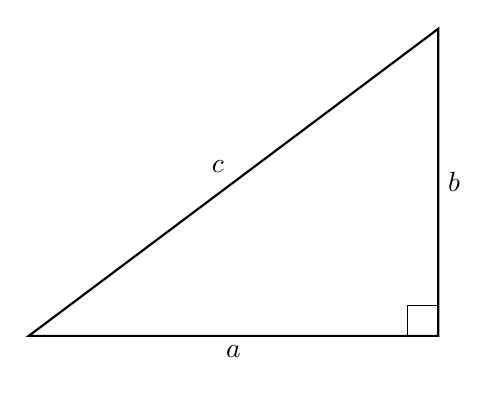
\begin{tikzpicture}[scale=1.3]
	\draw[thick] (0,0) -- (4,0) -- (4,3) -- cycle;
	\draw (3.7,0) -- (3.7,0.3) -- (4,0.3);		% pravý úhel
	\node[below] at (2,0) {$a$};
	\node[right] at (4,1.5) {$b$};
	\node[above left] at (2,1.5) {$c$};
\end{tikzpicture}
\end{center}

\textbf{Vývojový diagram} – jednoduchý flowchart:
\begin{center}
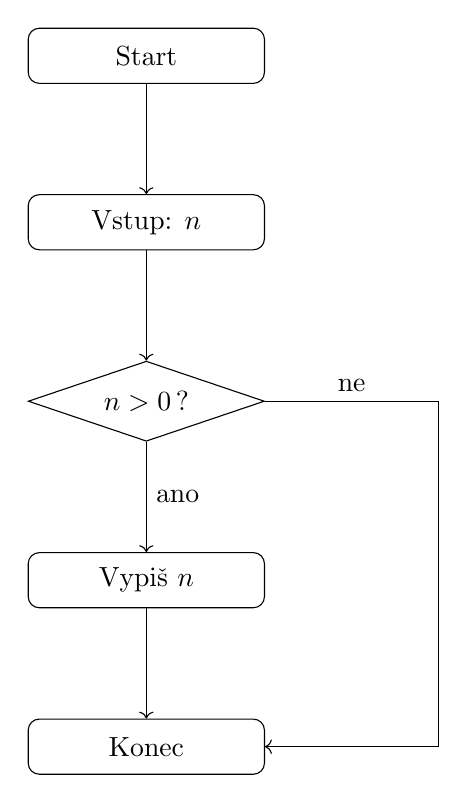
\begin{tikzpicture}[
	node distance=1.4cm,
	box/.style={rectangle, draw, rounded corners, minimum width=3cm,
	            minimum height=0.7cm, text centered},
	dec/.style={diamond, draw, minimum width=3cm, minimum height=0.7cm,
	            text centered, aspect=2.5}
]
	\node[box] (start) {Start};
	\node[box, below=of start] (vstup) {Vstup: $n$};
	\node[dec, below=of vstup] (podm) {$n > 0$\,?};
	\node[box, below=of podm] (vypis) {Vypiš $n$};
	\node[box, below=of vypis] (end) {Konec};
	\draw[->] (start) -- (vstup);
	\draw[->] (vstup) -- (podm);
	\draw[->] (podm) -- node[right] {ano} (vypis);
	\draw[->] (vypis) -- (end);
	\draw[->] (podm.east) -- node[above] {ne} ++(2.2,0) |- (end.east);
\end{tikzpicture}
\end{center}

% !TEX root = ../../vzor.tex
%% Ukázka: bloková schémata, UML diagram tříd, schéma databáze
%% Vkládá ji soubor vzor/kapitoly/prakticka.tex; ve vzor.pdf je pod nadpisem uvedeno „Zdroj ukázky".
%% Vyžaduje balíček tikz – v mprace.tex odkomentujte připravený řádek s \usepackage.

\section{Schémata programů}
\zdrojukazky{vzor/ukazky/schemata.tex}

Schémata jsou kreslená v \texttt{tikz} -- v souboru \texttt{mprace.tex}
odkomentujte řádek s \verb|\usepackage{tikz}|.

Dobrý popis složitějšího programu neobsahuje jen výpis kódu, ale také schéma struktury.
Schéma čtenáři rychle ukáže \emph{co} program dělá a \emph{jak} jsou jeho části propojeny
-- a vám pomůže promyslet architekturu \emph{před} psaním kódu.
Typické studentské projekty -- grafická hra, ovládání robota nebo zpracování dat
z fyzikálního pokusu -- mají vždy podobnou strukturu:
\textbf{vstupy}, \textbf{zpracování} a \textbf{výstupy}.
Právě tyto vztahy blokové schéma zachycuje.

\textbf{Jak sestavit blokové schéma:}
\begin{itemize}
	\item každý větší celek (modul, třída, soubor) = jeden blok
	\item šipky = tok dat nebo volání; na šipku napište \emph{co} teče nebo \emph{co} se volá
	\item datové soubory a herní stav odlište od modulů (jiný tvar nebo barva)
	\item schéma nemusí být úplné -- zachyťte hlavní vazby, ne každý řádek kódu
\end{itemize}

\textbf{Blokové schéma 1} -- procedurální program s datovými soubory (viz Příloha~B):

\begin{center}
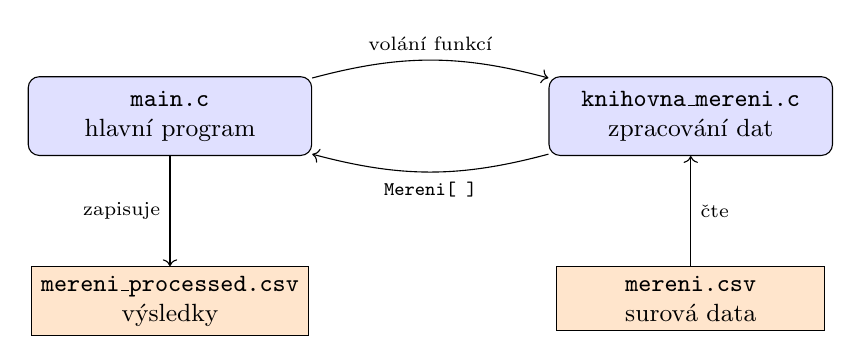
\begin{tikzpicture}[
	node distance=1.4cm and 3cm,
	modul/.style={rectangle, draw, rounded corners, fill=blue!12,
	              minimum width=3.6cm, minimum height=1cm,
	              align=center, font=\small},
	data/.style={rectangle, draw, fill=orange!20,
	             minimum width=3.4cm, minimum height=0.8cm,
	             align=center, font=\small}
]
	\node[modul] (main)  {\texttt{main.c}\\hlavní program};
	\node[modul, right=of main] (lib) {\texttt{knihovna\_mereni.c}\\zpracování dat};
	\node[data,  below=of main] (out) {\texttt{mereni\_processed.csv}\\výsledky};
	\node[data,  below=of lib]  (in)  {\texttt{mereni.csv}\\surová data};

	\draw[->, bend left=15] (main) to
		node[above, font=\scriptsize] {volání funkcí} (lib);
	\draw[->, bend left=15] (lib)  to
		node[below, font=\scriptsize] {\texttt{Mereni[ ]}} (main);
	\draw[->] (main) -- node[left,  font=\scriptsize] {zapisuje} (out);
	\draw[->] (in)   -- node[right, font=\scriptsize] {čte}      (lib);
\end{tikzpicture}
\end{center}

\textbf{Blokové schéma 2} -- architektura jednoduché hry (stejný princip platí
pro robotické projekty: vstupy\,=\,senzory, zpracování\,=\,mikrokontrolér, výstupy\,=\,motory):

\begin{center}
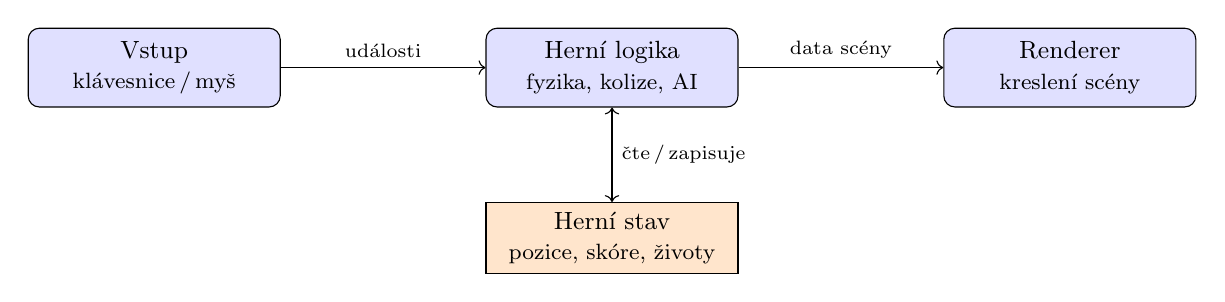
\begin{tikzpicture}[
	node distance=1.4cm and 2.6cm,
	modul/.style={rectangle, draw, rounded corners, fill=blue!12,
	              minimum width=3.2cm, minimum height=1cm,
	              align=center, font=\small},
	data/.style={rectangle, draw, fill=orange!20,
	             minimum width=3.2cm, minimum height=0.8cm,
	             align=center, font=\small}
]
	\node[modul] (vstup)  {Vstup\\{\footnotesize klávesnice\,/\,myš}};
	\node[modul, right=of vstup]  (logika) {Herní logika\\{\footnotesize fyzika, kolize, AI}};
	\node[modul, right=of logika] (render) {Renderer\\{\footnotesize kreslení scény}};
	\node[data,  below=1.2cm of logika] (stav) {Herní stav\\{\footnotesize pozice, skóre, životy}};

	\draw[->]  (vstup)  -- node[above, font=\scriptsize] {události}     (logika);
	\draw[->]  (logika) -- node[above, font=\scriptsize] {data scény}   (render);
	\draw[<->] (logika) -- node[right, font=\scriptsize] {čte\,/\,zapisuje} (stav);
\end{tikzpicture}
\end{center}

Pro složitější schémata, která se obtížně kreslí v \LaTeX{}u, lze použít nástroj
\href{https://www.diagrams.net}{draw.io} a výsledek vložit jako obrázek.

\textbf{UML diagram tříd} se hodí pro objektově orientovaný kód.
Každá třída má tři části: název, atributy (proměnné) a metody (funkce).
Viditelnost se značí \texttt{+} (veřejné) nebo \texttt{-} (privátní).
Šipka s dutým trojúhelníkem vyjadřuje \emph{dědičnost} -- odvozená třída
přebírá atributy a metody rodičovské třídy a může je rozšířit nebo přepsat:

\begin{center}
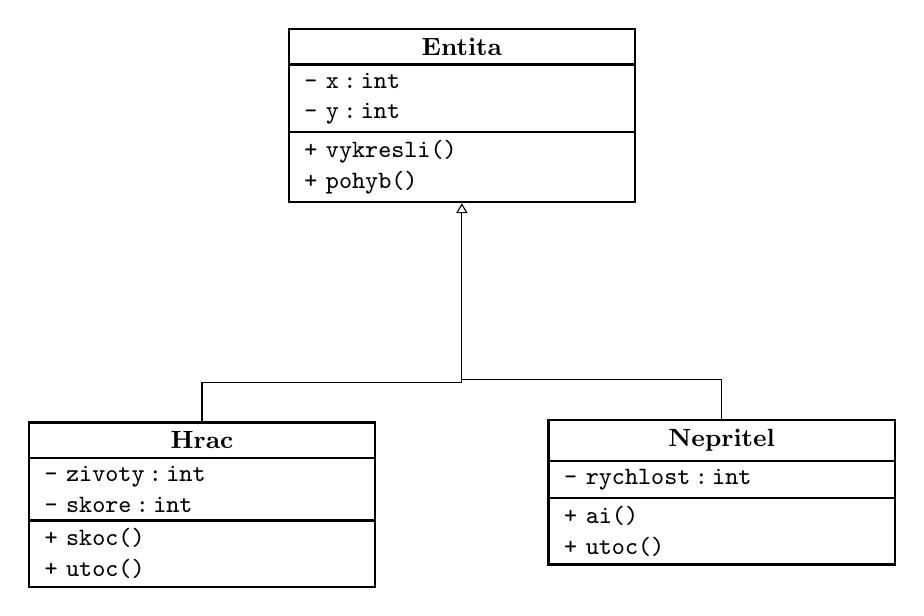
\begin{tikzpicture}[font=\small]
	%% Rodičovská třída Entita
	\node[draw, thick, minimum width=4.4cm, align=center, font=\small\bfseries]
		(en) {Entita};
	\node[draw, thick, minimum width=4.4cm, below=-\pgflinewidth of en,
	      align=left, text width=4.0cm, inner sep=3pt]
		(ena) {
			\texttt{- x\,:\,int}\\
			\texttt{- y\,:\,int}
		};
	\node[draw, thick, minimum width=4.4cm, below=-\pgflinewidth of ena,
	      align=left, text width=4.0cm, inner sep=3pt]
		(enm) {
			\texttt{+ vykresli()}\\
			\texttt{+ pohyb()}
		};
	%% Odvozená třída Hrac
	\node[draw, thick, minimum width=4.4cm, align=center, font=\small\bfseries]
		at (-3.3, -5) (hn) {Hrac};
	\node[draw, thick, minimum width=4.4cm, below=-\pgflinewidth of hn,
	      align=left, text width=4.0cm, inner sep=3pt]
		(hna) {
			\texttt{- zivoty\,:\,int}\\
			\texttt{- skore\,:\,int}
		};
	\node[draw, thick, minimum width=4.4cm, below=-\pgflinewidth of hna,
	      align=left, text width=4.0cm, inner sep=3pt]
		(hnm) {
			\texttt{+ skoc()}\\
			\texttt{+ utoc()}
		};
	%% Odvozená třída Nepritel
	\node[draw, thick, minimum width=4.4cm, align=center, font=\small\bfseries]
		at (3.3, -5) (nn) {Nepritel};
	\node[draw, thick, minimum width=4.4cm, below=-\pgflinewidth of nn,
	      align=left, text width=4.0cm, inner sep=3pt]
		(nna) {
			\texttt{- rychlost\,:\,int}
		};
	\node[draw, thick, minimum width=4.4cm, below=-\pgflinewidth of nna,
	      align=left, text width=4.0cm, inner sep=3pt]
		(nnm) {
			\texttt{+ ai()}\\
			\texttt{+ utoc()}
		};
	%% Šipky dědičnosti (dutý trojúhelník = generalizace)
	\coordinate (spoj) at (0, -3.7);
	\draw (hn.north) -- ++(0, 0.5) -| (spoj);
	\draw (nn.north) -- ++(0, 0.5) -| (spoj);
	\draw[-{Triangle[open]}] (spoj) -- (enm.south);
\end{tikzpicture}
\end{center}

\textbf{Schéma relační databáze} má podobnou strukturu jako UML diagram tříd,
ale místo metod obsahuje datové typy sloupců.
Primární klíč (\textit{PK}) jednoznačně identifikuje každý záznam;
cizí klíč (\textit{FK}) odkazuje na primární klíč jiné tabulky.
Šipka s popiskem \textit{N\,:\,1} vyjadřuje, že jeden hráč může mít více rekordů:

\begin{center}
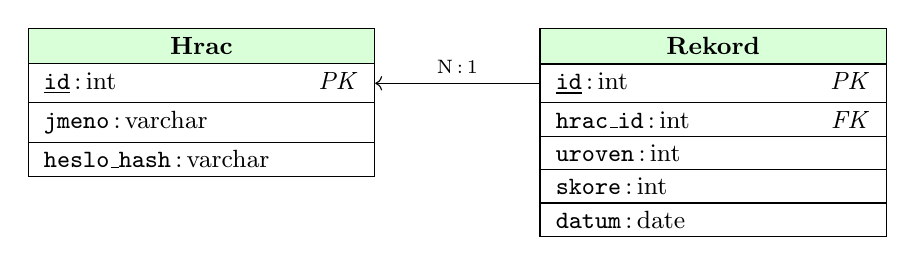
\begin{tikzpicture}[font=\small]
	%% Tabulka Hrac
	\node[draw, fill=green!15, minimum width=4.4cm, align=center,
	      font=\small\bfseries] (h0) {Hrac};
	\node[draw, minimum width=4.4cm, below=-\pgflinewidth of h0,
	      align=left, text width=4.0cm, inner sep=3pt]
		(h1) {\underline{\texttt{id}}\,:\,int\hfill\textit{PK}};
	\node[draw, minimum width=4.4cm, below=-\pgflinewidth of h1,
	      align=left, text width=4.0cm, inner sep=3pt]
		(h2) {\texttt{jmeno}\,:\,varchar};
	\node[draw, minimum width=4.4cm, below=-\pgflinewidth of h2,
	      align=left, text width=4.0cm, inner sep=3pt]
		(h3) {\texttt{heslo\_hash}\,:\,varchar};
	%% Tabulka Rekord
	\node[draw, fill=green!15, minimum width=4.4cm, align=center,
	      font=\small\bfseries] at (6.5, 0) (r0) {Rekord};
	\node[draw, minimum width=4.4cm, below=-\pgflinewidth of r0,
	      align=left, text width=4.0cm, inner sep=3pt]
		(r1) {\underline{\texttt{id}}\,:\,int\hfill\textit{PK}};
	\node[draw, minimum width=4.4cm, below=-\pgflinewidth of r1,
	      align=left, text width=4.0cm, inner sep=3pt]
		(r2) {\texttt{hrac\_id}\,:\,int\hfill\textit{FK}};
	\node[draw, minimum width=4.4cm, below=-\pgflinewidth of r2,
	      align=left, text width=4.0cm, inner sep=3pt]
		(r3) {\texttt{uroven}\,:\,int};
	\node[draw, minimum width=4.4cm, below=-\pgflinewidth of r3,
	      align=left, text width=4.0cm, inner sep=3pt]
		(r4) {\texttt{skore}\,:\,int};
	\node[draw, minimum width=4.4cm, below=-\pgflinewidth of r4,
	      align=left, text width=4.0cm, inner sep=3pt]
		(r5) {\texttt{datum}\,:\,date};
	%% Relace FK → PK  (trasa: nahoru pak doleva)
	\draw[->] (r2.west) |-
		node[pos=0.75, above, font=\scriptsize] {N\,:\,1} (h1.east);
\end{tikzpicture}
\end{center}

% !TEX root = ../../vzor.tex
%% Ukázka: výpisy programů (listings)
%% Vkládá ji soubor vzor/kapitoly/prakticka.tex; ve vzor.pdf je pod nadpisem uvedeno „Zdroj ukázky".

\section{Výpisy použitých programů}
\zdrojukazky{vzor/ukazky/vypisy.tex}

\lipsum[1]

Výpis programu \nameref{lst:hello_world_py} naleznete ve výpise \ref{lst:hello_world_py}.

\begin{lstlisting}[title={Program hello.py}, caption={hello.py}, label={lst:hello_world_py}]
# testovací program v Pythonu hello.py
# příliš žluťoučký kůň úpěl ďábelské ódy
CISLO = 10
i = CISLO

print("Hello World!")
print("Ahoj Světe!")
print(f"{i:d}")

#  END FILE
\end{lstlisting}

\lipsum[1]

\begin{lstlisting}[numbers=none, title={Příklad výstupního souboru}]
11.0524
5.5954
6.7996
13.8584
15.1357
Soucet: 52.4415
\end{lstlisting}

Seznam všech výpisů vytvoří příkaz \verb|\lstlistoflistings|
(v souboru \texttt{mprace.tex} je připravený, stačí ho odkomentovat).



% !TEX root = ../../vzor.tex
%% Závěr vzoru.
\chapter*{Závěr}
\addcontentsline{toc}{chapter}{Závěr}

\lipsum[1]


%% ---- SEZNAMY (vytvářejí se automaticky; nepotřebné smažte) ----
\printbibliography[heading=bibintoc]		% Seznam literatury
\listoffigures								% Seznam obrázků
\listoftables								% Seznam tabulek
% \lstlistoflistings						% Seznam výpisů programů

%% ---- PŘÍLOHY ----
\begin{appendices}
% !TEX root = ../../vzor.tex
%% Přílohy vzoru – ukázka je ve vzor/ukazky/prilohy.tex.
% !TEX root = ../../vzor.tex
%% Ukázka: přílohy (fotky z pokusů, seznam souborů v archivu)
%% Vkládá ji soubor vzor/kapitoly/prilohy.tex; ve vzor.pdf je pod nadpisem uvedeno „Zdroj ukázky".

\chapter{Fotky z pokusů}	
\zdrojukazky{vzor/ukazky/prilohy.tex}
\lipsum[1]
\chapter{Seznam souborů v přiloženém archivu}
V přiloženém archivu \texttt{novak\_vaclav\_4A.zip} naleznete následující soubory:

\begin{center}
\begin{tabular}{@{}l@{\,\dotfill\;}l@{}}
	\texttt{src/main.c}                    & hlavní program projektu \\
	\texttt{src/knihovna\_mereni.c}         & definice funkcí pro zpracování měření \\
	\texttt{data/mereni.csv}                & surová data měření \\
	\texttt{data/mereni\_processed.csv}     & zpracovaná data měření \\
\end{tabular}
\end{center}


\end{appendices}

\end{document}
